\subsection{Speisungen}
\label{subsec:Detailkonzept_Speisungen}

Wie dem Grobkonzept in Kapitel \ref{subsec:Blockschaltbild} entnommen werden kann, werden für das System vier verschiedene Speisungen benötigt. Es handelt sich dabei um eine 48V-, eine 12V-, eine 5V- und eine 3.3V Spannungsquelle. Auf diese Speisungen und deren Realisierung wird in den folgenden Unterkapiteln eingegangen. 

\subsubsection{48V Speisung}\label{subsubsec:48V_Speisung}

Um die benötigten 48V des Motors sicher zu stellen, wird ein fertiges Netzteil extern eingekauft. Auch alle weiteren Speisungen werden aus den 48V generiert.  Dabei muss jedoch abgeschätzt werden, wie viel Leistung dieses 48V Netzteil zur Verfügung stellen muss. Dazu wird in folgender Auflistung eine Leistungsabschätzung gemacht.

\begin{tabularx}{\textwidth}{llllllX}
 \textbf{Bauteil}& \textbf{Beschreibung} & \textbf{Referenz} & \textbf{U} & \textbf{Max. I} \\
\hline
Motor & Stillstandstrom & \cite[S.4]{sigmatec_servomotoren_2018}& 48V & I$_S$ & = & 5.41A 
\\
 & Nennstrom & \cite[S.4]{sigmatec_servomotoren_2018} & 48V & I$_N$ & = & 5.21A\\
\\
TMC6200 & Motorspannung & \cite[S.36]{trinamic_tmc6200_datasheet_2013}& 48V & I$_{V_S}$(24V) & = & 7mA \\
 & Analog Versorgung & \cite[S.36]{trinamic_tmc6200_datasheet_2013} & 12V & I$_{V_{SA}}$(24V) & = & 8mA\\
 & IC Versorgung & \cite[S.36]{trinamic_tmc6200_datasheet_2013} & 3.3V/5V & I$_{V_{CC}}$(5V) & = & 6mA\\
 & Digital Versorgung & \cite[S.36]{trinamic_tmc6200_datasheet_2013} & 3.3V/5V& I$_{V_{IO}}$(5V) & = & 30uA\\
 \\
TMC4671 & IC Versorgung & \cite[S.140]{trinamic_datasheet_2018} & 3.3V & I$_{IO}$ & = & k.A \\
 & Analog Referenz & \cite[S.141]{trinamic_datasheet_2018} & 5V & U$_{Ref}$ & = & 5V \\
\\
Resolver & TCA0372 Versorgung & \cite[S.3]{on_semiconductor_operational_2020}& 5V & I(25$^\circ C$) & = & 14mA \\
 & TCA0372 Output & & 5V & $I_{Spule}$ & = & 90mA\\
 & MC33202 & \cite[S.3]{on_semiconductor_low_2018}& 5V & I(25$^\circ C$) & = & 2.25mA \\
\\
Mikrocontroller & IC Versorgung & \cite[S.355]{atmel_8-bit_2014}& 5V & I$_{V_{max}}$ & = & 200mA \\
\\
Level-Shifter & IC Versorgung & \cite[S.3]{nxp_semiconductors_74hc4050_2016} & 3.3V & I$_{V_{max}}$ & = & 150mA\\
\\
ESP32 & IC Versorgung & \cite[S.21]{espressif_systems_esp32_2020}& 3.3V & I$_{V_{max}}$ & = & 68mA\\
\\
Display & Versorgung  & \cite{patrick_nx8048t070_nodate}& 5V & I$_{V_{max}}$ & = & 510mA\\
\\
Pumpen & Arbeitsspannung  & \cite{aiyimaindustrial_store_us_nodate}& 12V & I$_{V_{max}}$ &  = & 600mA\\
\\
Durchflusssensor & Versorgung  & \cite{five_+_tools_store_us_nodate}& 5V & I$_{V_{max}}$ &  = & 15mA\\
\\
\end{tabularx}

Die grossen Verbraucher, welche in das Gewicht fallen, sind in diesem Fall die Pumpen, das Display und der Förderbandmotor. Beim Förderbandmotor muss jedoch auch beachtet werden, dass dieser niemals unter Vollbelastung arbeiten wird. Auch bei den Pumpen wird jeweils immer nur eine arbeiten. Somit ergibt sich eine Leistung von ca. 16.44W für alle Komponenten ohne den Motor. Dies beinhaltet eine Pumpe, zwölf Durchflussmessgeräte, das Display und alle integrierten Schaltkreise. Da der Motor nie unter Vollast arbeiten wird, wird mit maximal 2A Arbeitsstrom gerechnet. Dies ergibt zusätzlich eine Leistung von 96W bei 48V. 

Um auf der sicheren Seite zu sein wird daher ein Netzteil benötigt, welches bei 48V ca. 150W Leistung liefert. Dies entspricht bei 100\% Wirkungsgrad der einzelnen Bauteile einem Ausgangsstrom von 3,125A. Eingesetzt  wird ein 48V/500W Netzteil von Aliexpress. Der Grund für diese Überdimensionierung ist, dass der Preis sich lediglich um 2CHF unterscheidet und man auf diese Weise in jedem Fall abgesichert ist. Dieses kann in Abbildung \ref{fig:Netzteil48V} begutachtet werden. \cite{aliexpress_us_nodate}.

\begin{figure}[h!]
	\centering
	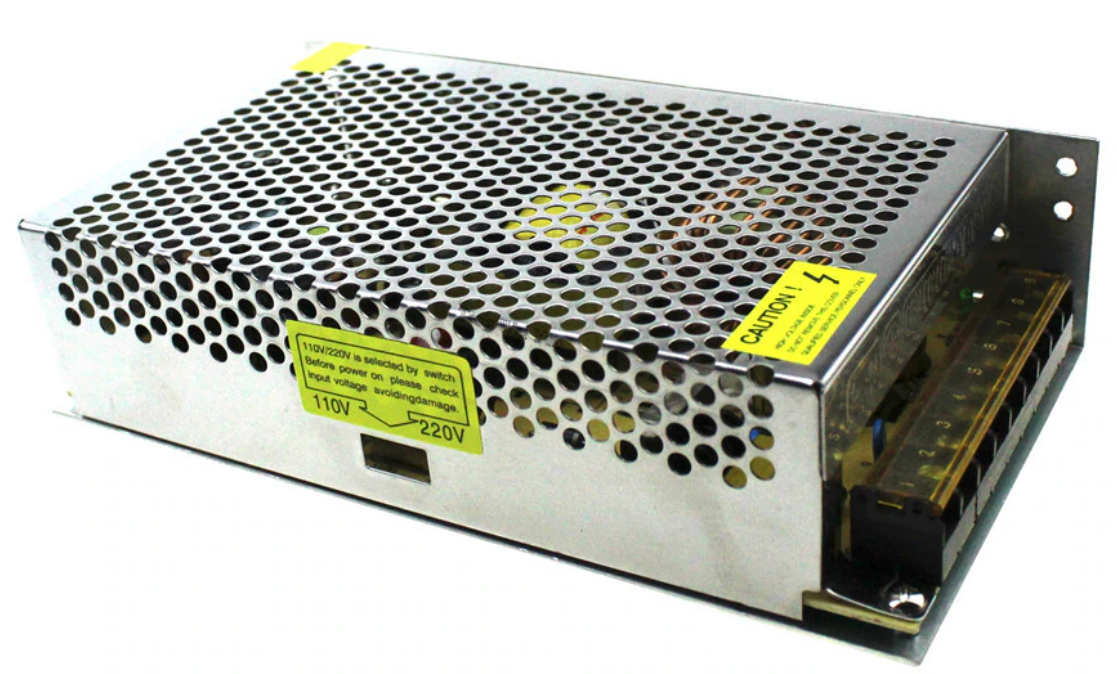
\includegraphics[width=0.8\textwidth]{graphics/Netzteil48V.png}
	\caption{Ansichtsbild des 48V Netzteils \cite{aliexpress_us_nodate}.}
	\label{fig:Netzteil48V}
\end{figure} 

\subsubsection{12V Speisung}\label{subsubsec:12V_Speisung}

Die 12V Speisung wird mittels Schaltspannungsregler realisiert. Es handelt sich hierbei um einen Regler von Monolithic Power Systems. Genauer gesagt um den MP24943DN-LF. Die Auswahl ist auf dieses Bauteil gefallen, da eine relativ hohe Eingangsspannung von 48V verarbeitet werden muss. Der MP24943DN-LF kann am Eingang mit Spannungen von 4.5-55V arbeiten und dabei eine Ausgangsspannung von 0.8-45V erzeugen. Dies bei einem maximalen Strom von bis zu 3A. Die Realisierung der 12V Speisung kann in Abbildung \ref{fig:12VSpeisung_Schema} betrachtet werden. \cite{mouser_mp24943dn-lf_nodate}

\begin{figure}[h!]
	\centering
	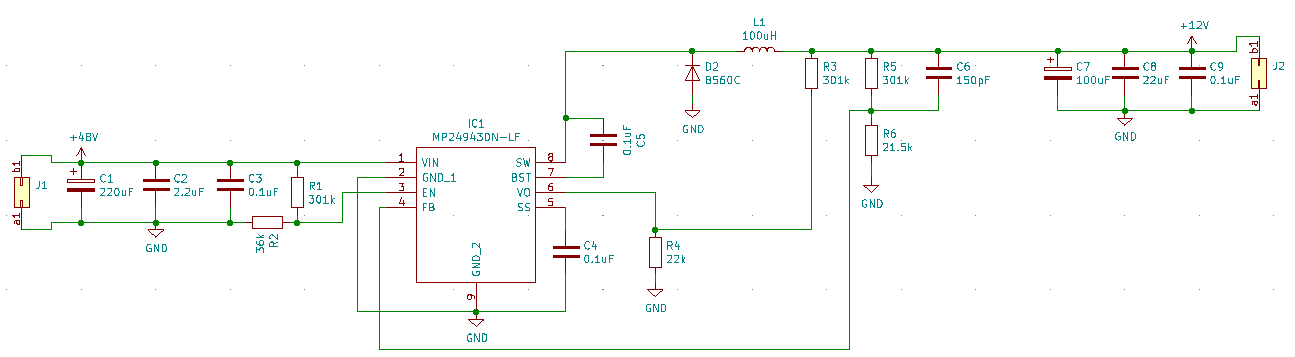
\includegraphics[width=\textwidth]{graphics/12V_Speisung_Schema.png}
	\caption{Schema der 12V Speisung}
	\label{fig:12VSpeisung_Schema}
\end{figure}  
\newpage
Bei den Kondensatoren C1-C3 handelt es sich um Filterkondensatoren, welche hochfrequente Störungen der Eingangsspannung von 48V glätten. Der Enable Eingang wird mit dem Spannungsteiler R1 \& R2 auf aktiv gesetzt. \cite{mouser_mp24943dn-lf_nodate}  

Die gewünschte Ausgangsspannung wird mittels Spannungsteiler R5 \& R6 eingestellt, welche auf den Feedback Eingang rückgekoppelt werden. Diese berechnet sich laut Datenblatt gemäss Formel \ref{equ:Ausgangsspannung_12V}. \cite{mouser_mp24943dn-lf_nodate}

\begin{align}
R6 &= \frac{R5}{\frac{Vout}{0.8}-1}
\label{equ:Ausgangsspannung_12V}
\end{align}

Bei einem Widerstandsverhältnis von R5=301k$\Omega$ \& R6=21.5k$\Omega$ entspricht dies einer Ausgangsspannung von 12V.

Um einer Überspannung vorbeugen zu können, wird am Eingang VO ein Spannungsteiler implementiert. Diese wird am VO-Eingang mit einer Referenzspannung von 0.9V verglichen. Übersteigt die Spannung an VO die Referenzspannung von 0.9V, so wird der Regler ausgeschaltet, bis die Spannung wieder unter 0.9V fällt. Als maximale Ausgangsspannung wurde hierbei eine Spannung von 13V gewählt. Diese Wahl wurde getroffen, da die 12V ausschliesslich für die Ansteuerung der Pumpen verwendet wird und diese eine Spannung von 13V verkraften können ohne Schaden zu nehmen. Der Spannungsteiler wird gemäss Datenblatt mit der Formel \ref{equ:Vovp_12V} berechnet. \cite{mouser_mp24943dn-lf_nodate}

\begin{align}
R4 &= \frac{R3}{\frac{Vovp}{Vovref}-1}
\label{equ:Vovp_12V}
\end{align}

Bei einem Widerstandsverhältnis von R3=301k$\Omega$ \& R4=22k$\Omega$ entspricht dies einer Überspannungsschutzschwelle von 13.21V. \cite{mouser_mp24943dn-lf_nodate}

Der Rippel des Spulenstroms lässt sich gemäss Formel \ref{equ:12V_Spulenberechnung} berechnen. Dieser sollte gemäss Datenblatt ca. 30\% des maximalen Ausgangsstroms von 3A betragen. \cite{mouser_mp24943dn-lf_nodate} 

\begin{align}
L1 &= \frac{Vout*(Vin-Vout)}{Vin*\Delta IL*fosc}
\label{equ:12V_Spulenberechnung}
\end{align}

Der interne Oszillator läuft dabei bei einer Frequenz von 100kHz. Bei der ausgewählten Spule von 100$\mu$H erhalten wir ein $\Delta$I$_{L}$ von 0.9A. Ausserdem wird im Datenblatt darauf hingewiesen, dass die gewählte Spule auf mindestens 125\% des maximalen Ausgangsstroms von 3A ausgelegt werden soll. Auch der Gleichstromwiederstand der Spule sollte $ \leq \ $ 200m$\Omega$  sein. \cite{mouser_mp24943dn-lf_nodate}

Mit den Kondensatoren C7, C8 \&C9 wird die Ausgangsspannung zum Abschluss noch geglättet. Bei den Eingangskondensatoren, sowie den Ausgangskondensatoren sollte es sich um low ESR Typen handeln. \cite{mouser_mp24943dn-lf_nodate}

\subsubsection{5V Speisung}
\label{subsubsec:5V_Speisung}

Bei der 5V Speisung wurde erneut auf den MP24943DN-LF von Monolithic Power Systems gesetzt. Die Beschaltung ist dabei die gleiche, wie bei der 12V Speisung. Der Unterschied ist jedoch, dass für die Ausgangsspannung und für die Überspannungsschwelle andere Widerstandsverhältnisse gewählt werden müssen. Auch die Spule muss anders ausgelegt werden. In Abbildung \ref{fig:5VSpeisung_Schema} ist das Schema der 5V Speisung zu sehen. \cite{mouser_mp24943dn-lf_nodate} 
 
\begin{figure}[h!]
\centering
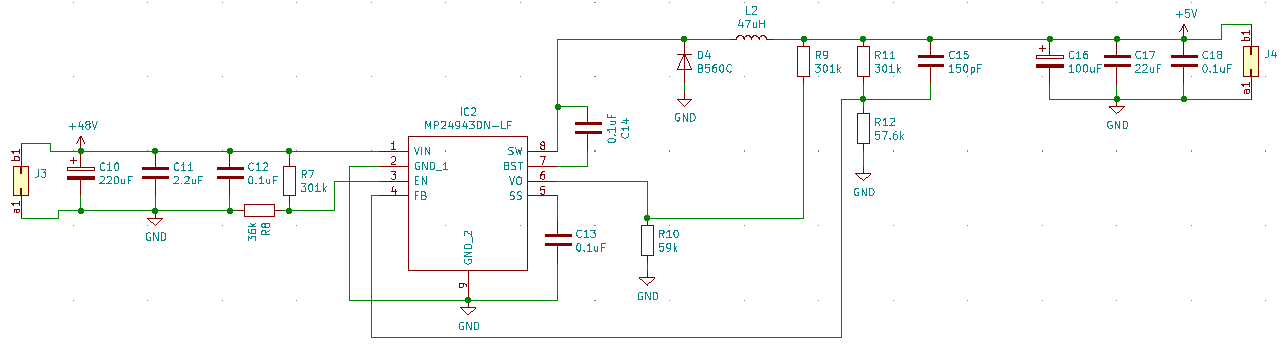
\includegraphics[width=\textwidth]{graphics/5V_Speisung_Schema.png}
\caption{Schema der 5V Speisung}
\label{fig:5VSpeisung_Schema}
\end{figure} 
 
Das Widerstandsverhältnis von R11 \& R12, welches die Ausgangsspannung definiert, wurde gemäss Formel \ref{equ:Ausgangsspannung_12V} berechnet. Somit ergeben sich für R11=301k$\Omega$ und für R12=57.6k$\Omega$, Was einer Ausgangsspannung von 4.98V entspricht. \cite{mouser_mp24943dn-lf_nodate}

Beim Überspannungsschutz muss darauf geachtet werden, dass der Mikrokontroller AtMega2560-16AU nur in einem Spannungsbereich von 4.5V-5.5V betrieben werden darf. Die maximal verträgliche Eingangsspannung liegt laut Datenblatt bei 6V. Somit muss der Überspannungsschutz so gestaltet werden, dass die Schwelle von 6V nicht überschritten werden kann. Um dies erreichen zu können, wurde für R9=301k$\Omega$ und R10=53k$\Omega$ gewählt. Gemäss Formel \ref{equ:Vovp_12V} erhält man so eine Überspannungsschutzschwelle von 6V. \cite{mouser_mp24943dn-lf_nodate}

Der interne Oszillator läuft wiederum bei einer Frequenz von 100kHz. Bei der ausgewählten Spule von 47$\mu$H erhalten wir ein $\Delta$I$_{L}$ von 0.953A. Auch hier gilt gemäss Datenblatt, dass die gewählte Spule auf mindestens 125\% des maximalen Ausgangsstroms von 3A ausgelegt werden soll. Auch der Gleichstromwiederstand der Spule sollte $ \leq \ $ 200m$\Omega$  sein. \cite{mouser_mp24943dn-lf_nodate} 

Mit den Kondensatoren C16, C17 \&C18 wird die Ausgangsspannung zum Abschluss noch geglättet. Bei den Eingangskondensatoren, sowie den Ausgangskondensatoren sollte es sich um low ESR Typen handeln. \cite{mouser_mp24943dn-lf_nodate}
\newpage
\subsubsection{3,3V Speisung}
\label{subsubsec:3,3V_Speisung}

Um die Treiber der Motorenansteuerung ansteuern zu können, wird zusätzlich eine 3,3V Speisung verbaut. Diese muss gemäss der Leistungsabschätzung in Kapitel  \ref{subsubsec:48V_Speisung} einen maximalen Strom von ca. 250mA liefern können. Dazu wird ein Linearregler eingesetzt, welcher von der 5V Speisung aus betrieben wird. Es handelt sich um den LF33CDT-TRY  von STMicroelectronics. Dieser hat eine fixe Ausgangsspannung von 3,3V, bei einem maximalen Strom von 1A. \cite{noauthor_very_nodate}